\documentclass{article}

\usepackage[utf8]{inputenc}
\usepackage{parskip}
\usepackage{amssymb,amsfonts,amsmath,amscd}
\usepackage{bm}
\usepackage{hyperref}
\usepackage[pdftex]{graphicx}
\usepackage{url}
\usepackage[usenames,dvipsnames]{color}
\usepackage{enumitem}
\usepackage{mathtools}
\usepackage{float}

% for typesetting in-text numbers and units
\usepackage{siunitx}

% Table stuff.
\usepackage{booktabs}
\usepackage{makecell}
\usepackage{multirow}

% biblatex for bibliography
\usepackage[
backend=biber,
maxcitenames=1,
style=authoryear,
]{biblatex}

% \addbibresource{bibliography.bib}

\DeclareMathOperator*{\argmin}{argmin}
\DeclareMathOperator*{\arctantwo}{\mathrm{arctan2}}

\title{Mobile Manipulation Calibration}
\author{Adam Heins}

\begin{document}

\maketitle

\section{Introduction}

The frames of interest are listed in Table~\ref{tab:frames}.

\begin{table}[h]
  \caption{Coordinate frames.}
  \centering
    \begin{tabular}{l c}
      \toprule
      Name & Subscript \\
      \midrule
      World        & $w$ \\
      Mobile base  & $b$ \\
      Base of arm  & $a$ \\
      End effector & $e$  \\
      Tool         & $t$ \\
      \bottomrule
    \end{tabular}
  \label{tab:frames}
\end{table}

The pose~$\bm{T}_{wt}$ of an arbitrary tool attached to the end effector can be
computed using the sequence of transforms
\begin{equation}\label{eq:kinematic_chain}
  \bm{T}_{wt} = \bm{T}_{wb}(\bm{q}_b)\bm{T}_{ba}\bm{T}_{ae}(\bm{q}_a)\bm{T}_{et},
\end{equation}
where~$\bm{T}_{wb}$ depends on the base
configuration~$\bm{q}_b=[x_b,y_b,\theta_b]^T$ and~$\bm{T}_{ae}$ depends on the
arm configuration~$\bm{q}_a$.

\section{Vicon Zero Pose}

The \texttt{vicon\_bridge} package allows one to provide a \emph{zero pose} to
specify the desired origin of a given model. Given the true robot frame~$\{r\}$
and the Vicon model frame~$\{v\}$, we have
\begin{equation*}
  \bm{T}_{wr} = \bm{T}_{wv}\bm{T}_{vr},
\end{equation*}
where~$\bm{T}_{vr}$ is a constant transform we need to calibrate. The zero
pose~$\bm{T}_{wv}^0$ is such that~$\bm{T}_{wr}=\bm{I}$, which
implies~$\bm{T}_{wv}^0\bm{T}_{vr}=\bm{I}$ and
thus
\begin{equation*}
  \bm{T}_{wv}^0 = \bm{T}_{vr}^{-1} = \begin{bmatrix} \bm{C}_{rv} & \bm{r}^{vr}_r \\ \bm{0}^T & 1 \end{bmatrix}
\end{equation*}

\section{Base Calibration}

\subsection{Center of Rotation}

We need to calibration the Vicon measured base poses~$\hat{\bm{T}}_{wv}$ so
that the origin of~$\bm{T}_{wb}$ is correct (i.e., we want it at the center of
rotation, such that there is no translational motion when the base is commanded
to rotate). Starting at an arbitrary configuration~$\hat{\bm{T}}_{wv,0}$, we
will move the base to a sequence of desired yaw angles~$\theta^d_i$ and obtain
the corresponding measured configurations~$\hat{\bm{T}}_{wv,i}$. We want to
find~$\bm{r}^{bv}_v$ such that~$\hat{\bm{r}}_{wb,i} = \hat{\bm{r}}_{wb,0}$ is
satisfied as closely as possible for each~$i$, which yields the least-squares
problem
\begin{equation}\label{eq:base_position_lstsq}
  \argmin_{\bm{r}^{bv}_v}\ \frac{1}{2}\sum_i\left\|\hat{\bm{C}}_{wv,i}\bm{r}^{bv}_v + \hat{\bm{r}}^{vw}_{w,i} - \hat{\bm{C}}_{wv,0}\hat{\bm{r}}^{bv}_{v} - \hat{\bm{r}}^{vw}_{w,0}\right\|^2.
\end{equation}
This gives us~$\bm{r}^{bv}_v$, but what we want for the Vicon zero pose is~$\bm{r}^{vb}_b=-\bm{C}_{bv}\bm{r}^{bv}_v$, so we need to negate the value and be careful to rotate it from the Vicon frame to the base frame if~$\bm{C}_{bv}\neq\bm{I}$.

We can write~\eqref{eq:base_position_lstsq} in the form~$\|\bm{A}\bm{x}-\bm{b}\|^2$ by taking~$\bm{x}=\bm{r}^{bv}_v$ and
\begin{align*}
  \bm{A} &= \begin{bmatrix}
    \hat{\bm{C}}_{wv,0} - \hat{\bm{C}}_{wv,0} \\ \vdots \\ \hat{\bm{C}}_{wv,n} - \hat{\bm{C}}_{wv,0}
  \end{bmatrix}, & \bm{b} = \begin{bmatrix}
  \hat{\bm{r}}^{vw}_{w,0} - \hat{\bm{r}}^{vw}_{w,0} \\ \vdots \\ \hat{\bm{r}}^{vw}_{w,0} - \hat{\bm{r}}^{vw}_{w,n}
  \end{bmatrix}.
\end{align*}

\subsection{Orientation (Yaw)}

We also need to calibrate the Vicon measured base poses~$\hat{\bm{T}}_{wv}$ so
that the yaw angle of the model is aligned with the actual forward direction
of~$\bm{T}_{wb}$; that is, the direction of pure forward velocity. Starting at
a particular pose~$\hat{\bm{T}}_{wv,0}$, we command the Ridgeback to drive
forward and periodically measure the pose~$\hat{\bm{T}}_{wv,i}$. Ideally, the
position of the base would be aligned with the $x$-axis of the initial frame.
Let~$\bm{p}_i=\bm{C}_{wv,0}^T(\bm{r}^{vw}_{w,i}-\bm{r}^{vw}_{w,0})$. The yaw
error is~$\Delta\theta_i=\arctantwo(p_{y,i},p_{x,i})$. We then solve the problem
\begin{equation}\label{eq:base_yaw_lstsq}
  \argmin_{\theta_{vb}}\ \frac{1}{2}\sum_i(\theta_{vb}-\Delta\theta_i)^2,
\end{equation}
with corresponding Vicon zero orientation~$\bm{C}_{bv}=\bm{C}_z(-\theta_{vb})$.

\textbf{Important:} remember to take this into account when computing the
overall base zero pose including the position, as discussed above.

We can write~\eqref{eq:base_yaw_lstsq} in the
form~$\|\bm{A}x-\bm{b}\|^2$ by taking~$x=\theta_{bv}$,~$\bm{A}$ a vector of
ones, and~$\bm{b}$ a vector of the angle errors~$\Delta\theta_i$.

\section{Arm--End Effector--Tool Calibration}

\begin{figure}[h]
  \centering
  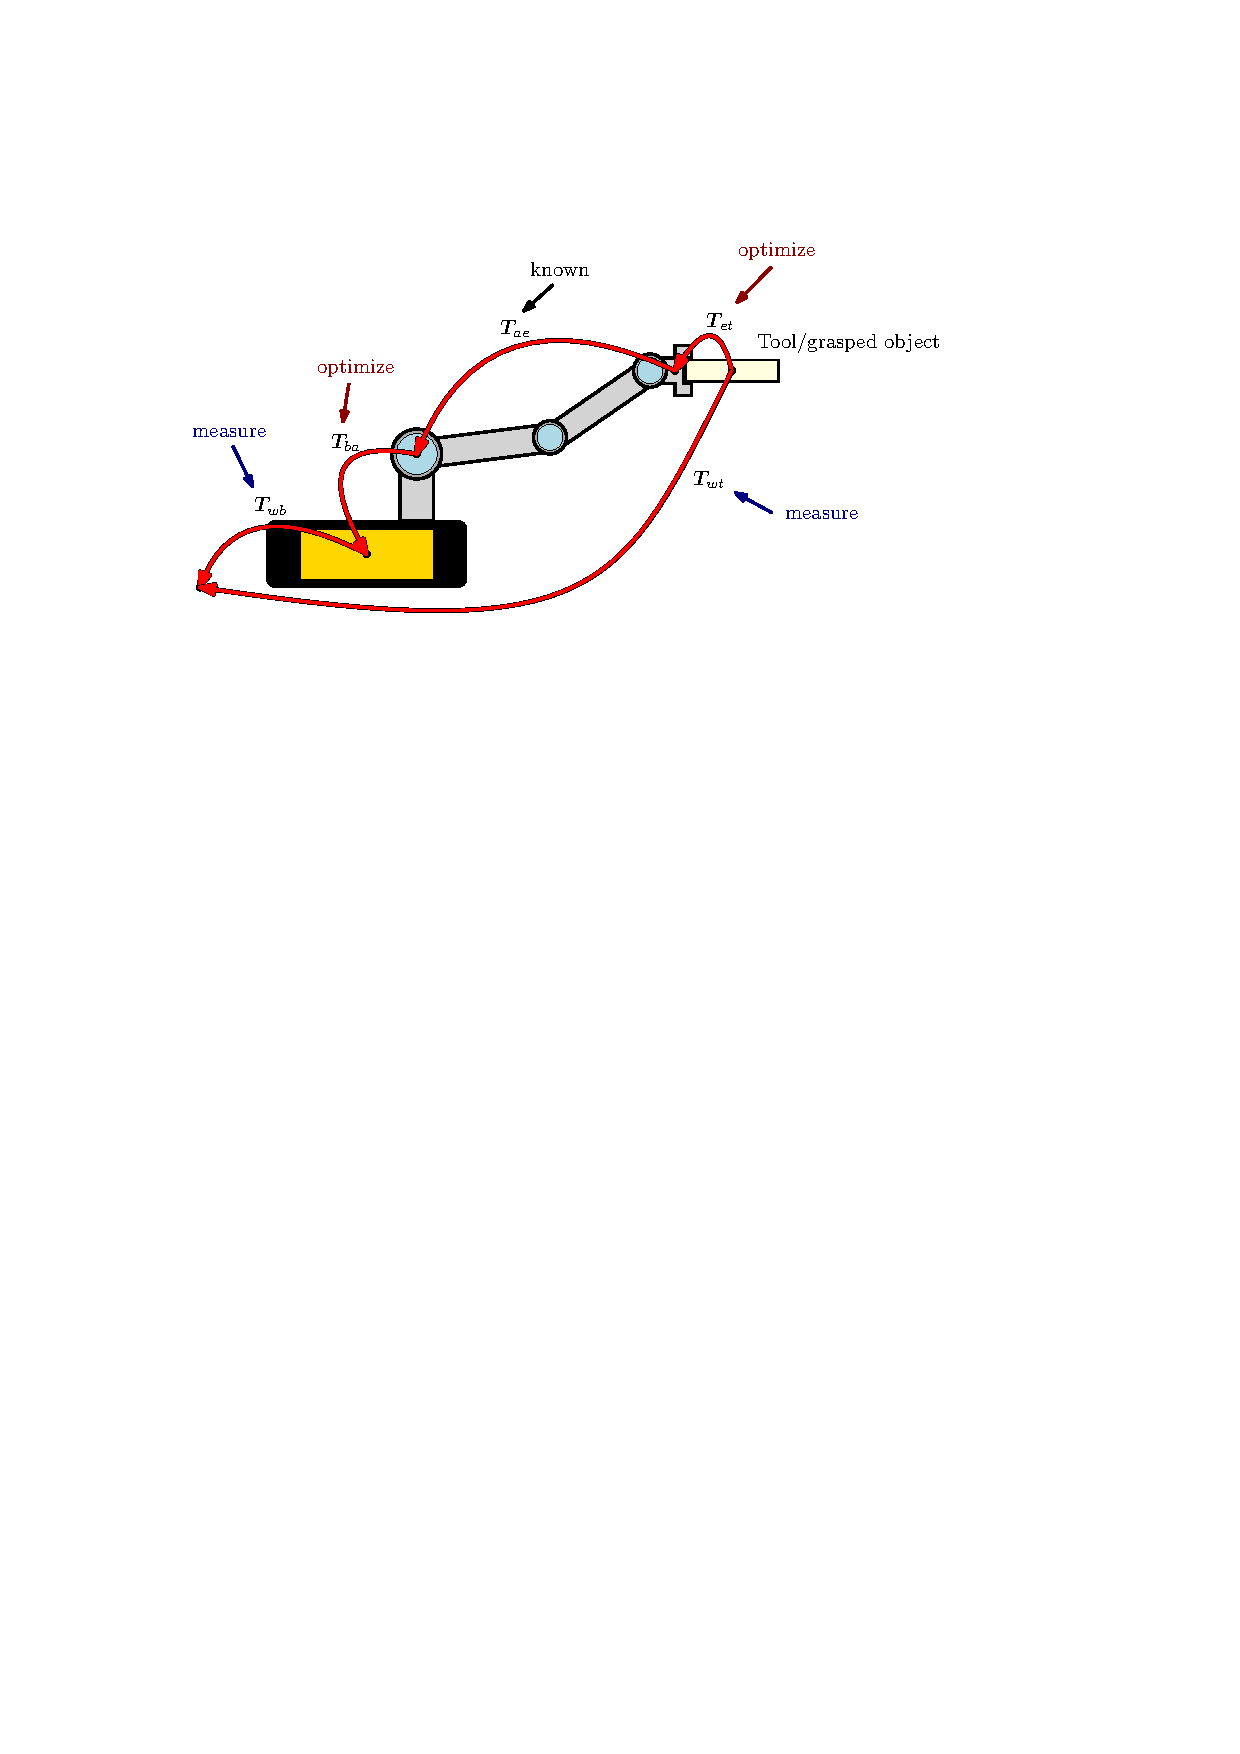
\includegraphics[width=1\textwidth]{figures/robot_calibration.pdf}
  \caption{Frames on the robot being calibrated.}
    \label{fig:calibration}
\end{figure}

Having calibrated the base pose~$\bm{T}_{wb}$, we now wish to calibrate
(static) the transforms between the base and arm~$\bm{T}_{ba}$ and the EE and
tool~$\bm{T}_{et}$. We will assume that factory calibration for the arm
transform~$\bm{T}_{ae}(\bm{q}_a)$ is good enough.

To do so, we will collect a sequence of
pairs~$(\bm{q}_{a,i},\hat{\bm{T}}_{wt,i})$ by moving the arm to the sequence of
configurations~$\bm{q}_{a,i}$. We will then solve the (nonlinear) least squares
problem
\begin{equation}
  \argmin_{\bm{T}_{ba},\bm{T}_{wt}}\ \frac{1}{2}\sum_i\|\boxminus(\bm{T}_{wt}(\bm{q}),\hat{\bm{T}}_{wt})\|^2.
\end{equation}
over the manifold~$SE(3)$, where~$\bm{T}_{wt}$ is computed using~\eqref{eq:kinematic_chain} and
\begin{equation}
  \boxminus(\bm{T}_1,\bm{T}_2) = \log(\bm{T}_1^{-1}\bm{T}_2)^\vee
\end{equation}
is the error between the poses. We can include any prior information about the
transforms as an initial guess for the solver.

\section{Force Sensor Calibration}

Here our goal is to find the orientation~$\bm{C}_{bf}$ of the force sensor
frame~$\{f\}$ about the $x$- and $y$-axes of a frame~$\{b\}$ with a gravity-aligned
$z$-axis. To do so, we will zero the sensor and then attach a mass~$m$ to it
and collect a set of force measurements~$\{\bm{f}_{f,i}\}_{i=1}^n$. We then
solve the nonlinear least-squares problem
\begin{equation*}
  \argmin_{\Delta\bm{C}\in SO(3)} \frac{1}{2}\sum_i\|\Delta\bm{C}\bar{\bm{C}}_{bf}\bm{f}_{f,i}-m\bm{g}\|^2
\end{equation*}
for the orientation offset~$\Delta\bm{C}$ such
that~$\bm{C}_{bf}=\Delta\bm{C}\bar{\bm{C}}_{bf}$ with~$\bar{\bm{C}}_{bf}$ a
nominal guess for the orientation.

Calibrating the yaw angle offset would be more complicated, and at least
require multiple orientations of~$\bm{C}_{bf}$ to identify.

\end{document}
